\documentclass[twoside, final]{hcmut_report}

% Configuration
\newcommand{\var}[1]{\textbf{#1}}
\upperuniname{VIETNAM NATIONAL UNIVERSITY HO CHI MINH CITY}
\uniname{HO CHI MINH CITY UNIVERSITY OF TECHNOLOGY}
\deptname{FACULTY OF COMPUTER SCIENCE AND ENGINEERING}

\coursename{\LARGE Microcontrollers \\ \large (CO3117)}
\reporttype{\Large Report Lab 2}
\title{\Large TIMER AND INTERRUPT}

\advisor{
TS. Lê Trọng Nhân
}
\student{
   Nguyễn Chí Thanh, 2313078
}
\setlength{\parindent}{2em}
\begin{document}
\coverpage
\pagestyle{empty}
\tableofcontents
\pagestyle{fancy}
\pagebreak
\section{Introduction}
In this lab, we will explore various LED animations using a microcontroller. The goal is to understand how to control LEDs and create visually appealing effects.
This report consists of:
\begin{itemize}
    \item Source code C language for LED animations in STM32CubeIDE.
    \item Simulate LED animations using Proteus software.
\end{itemize}
For more details about source code, visit my \href{https://batmaon512.github.io/Microcontroller-251}{GitHub repository}.

\section{Exercise and Report}
\subsection{Exercise 1}
The first exercise show how to interface for multiple seven segment LEDs to STM32F103C6 micro-controller (MCU). Seven segment displays are common anode type, meaning that the anode of all LEDs are tied together as a single terminal and cathodes are left alone as individual pins. \\

In order to save the resource of the MCU, individual cathode pins from all the seven segment LEDs are connected together, and connect to 7 pins of the MCU. These pins are popular known as the \textbf{signal pins}. Meanwhile, the anode pin of each seven segment LEDs are controlled under a power enabling circuit, for instance, an PNP transistor. At a given time, only one seven segment LED is turned on. However, if the delay is small enough, it seems that all LEDs are enabling. \\

Implement the circuit simulation in Proteus with two 7-SEGMENT LEDs as following:

\begin{figure}[!htp]
    \centering
    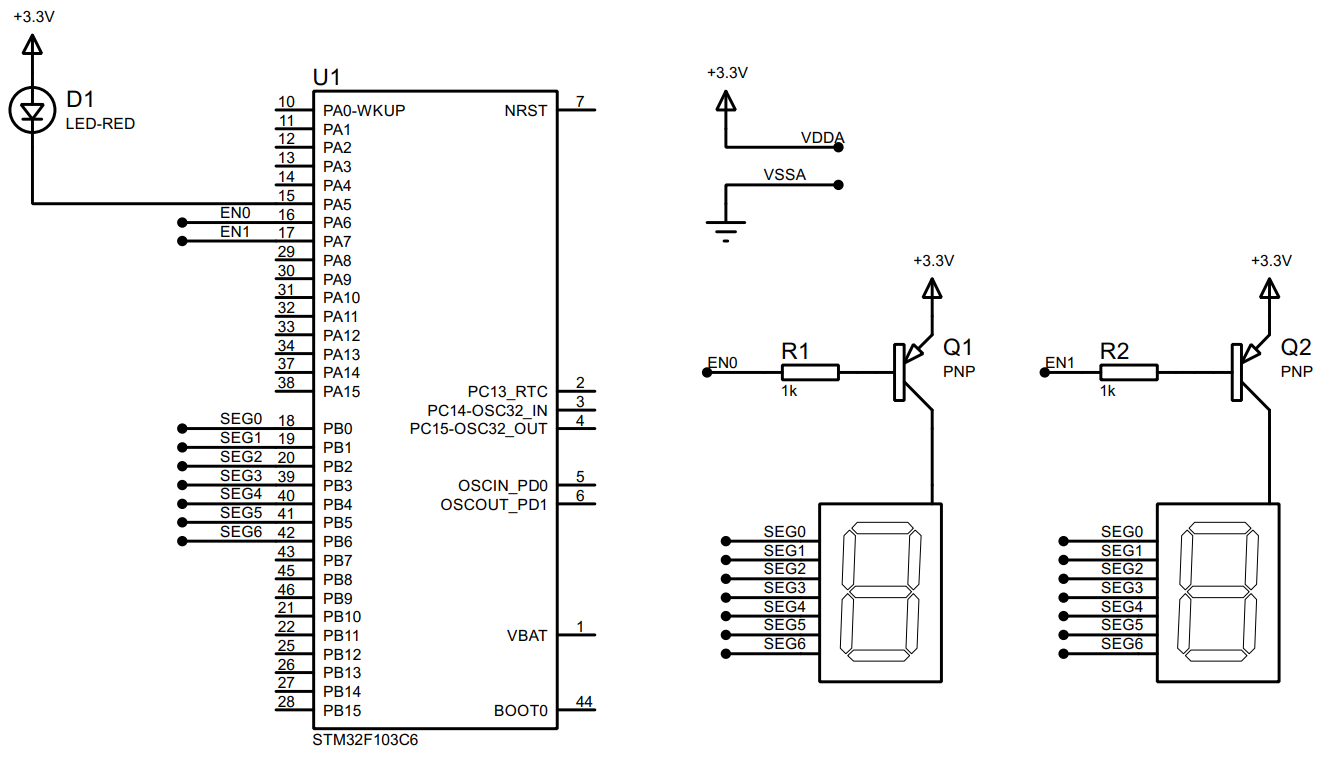
\includegraphics[width=5.5in]{graphics/lab2_ex1a.PNG}
    \caption{\textit{Simulation schematic in Proteus}}
    \label{bai2_pic1a}
\end{figure}
Components used in the schematic are listed bellow:
\begin{itemize}
    \item 7SEG-COM-ANODE (connected from PB0 to PB6)
    \item LED-RED
    \item PNP
    \item RES
    \item STM32F103C6
\end{itemize}


Students are proposed to use the function \textbf{display7SEG(int num)} in the Lab 1 in this exercise. Implement the source code in the interrupt callback function to display number \textbf{"1"} on the first seven segment and number \textbf{"2"} for second one. The switching time between 2 LEDs is half of second. \\

\textbf{Report 1: } Capture your schematic from Proteus and show in the report.\\
\begin{figure}[!htp]
    \centering
    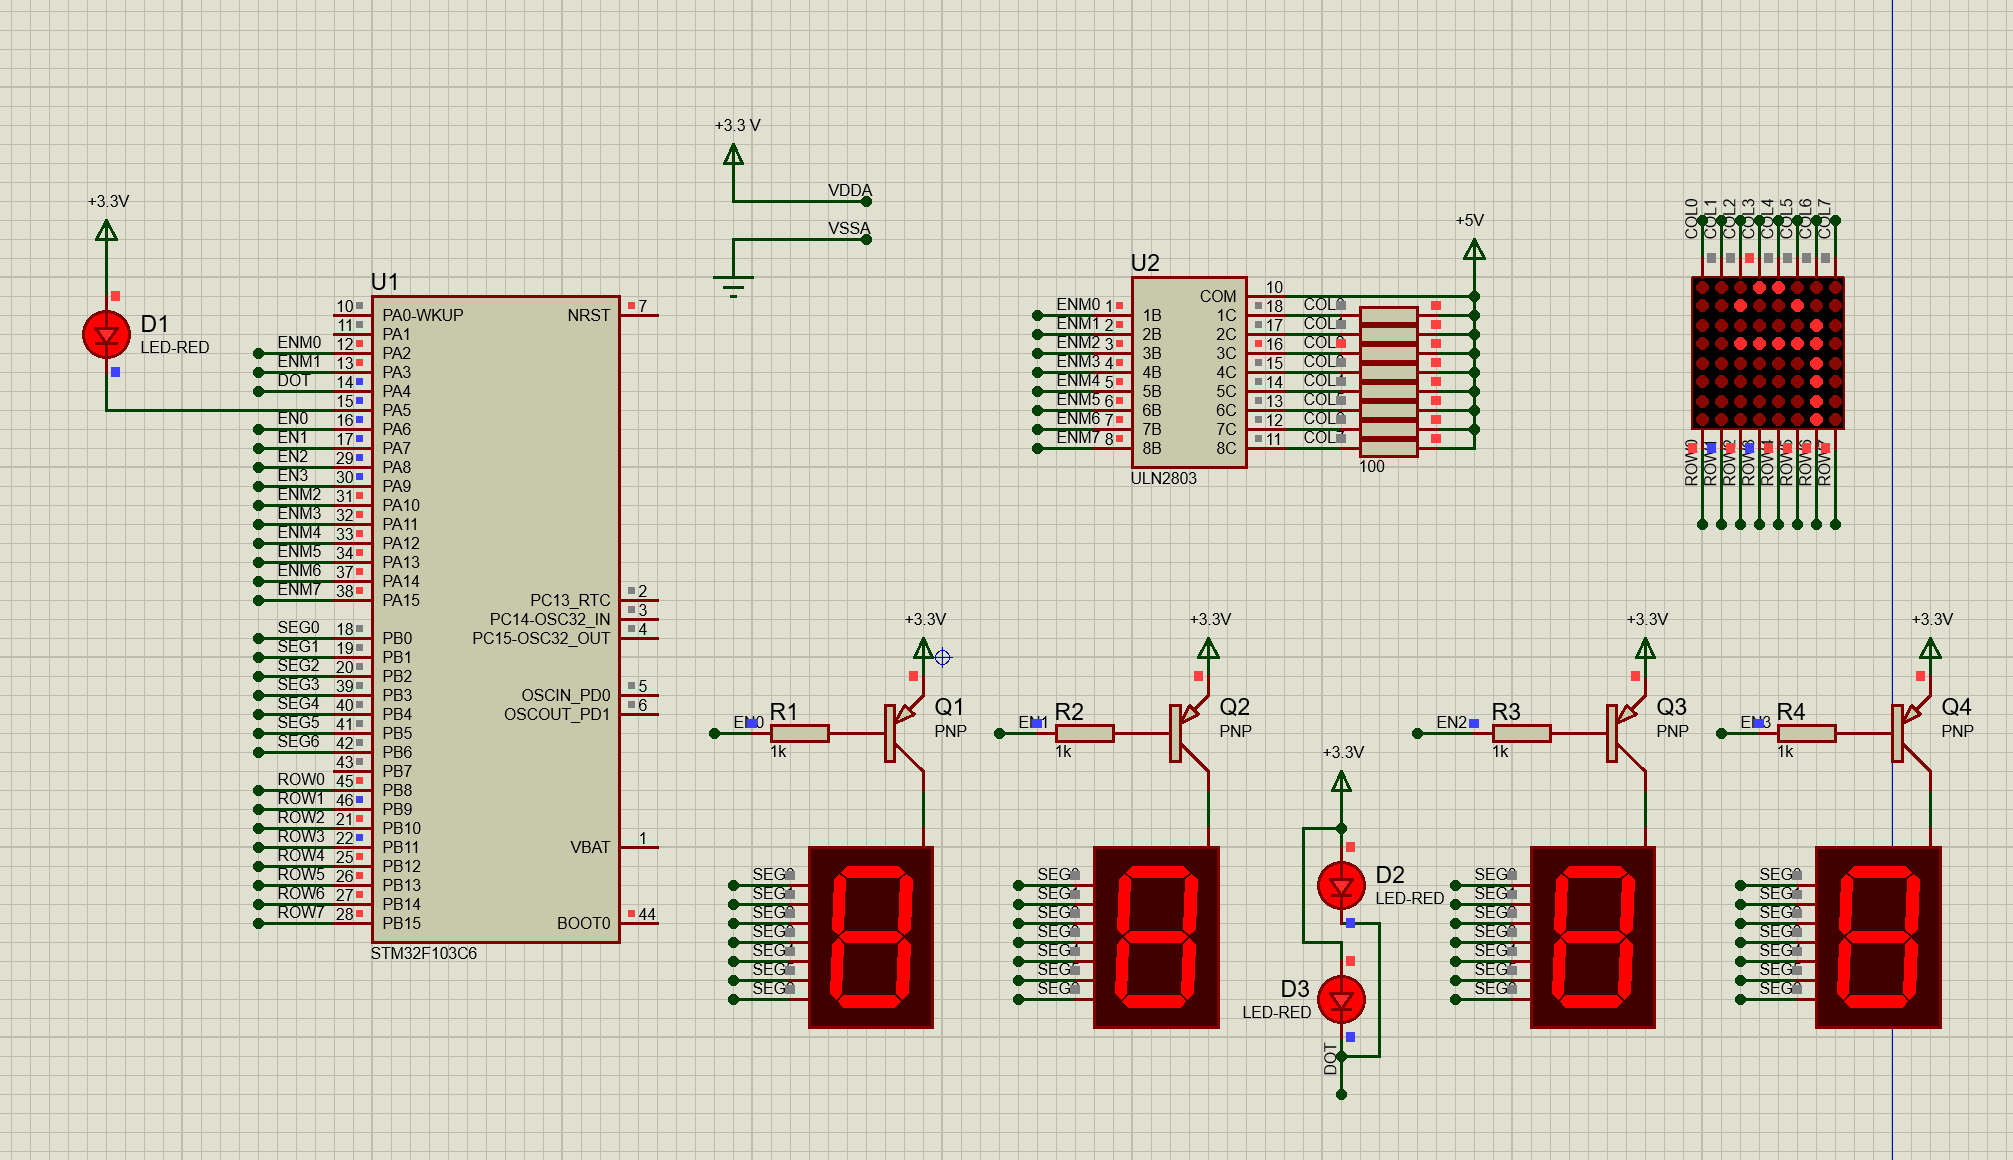
\includegraphics[width=5.5in]{graphics/f1.png}
    \caption{\textit{Schematic in Proteus}}
\end{figure}

\pagebreak
\textbf{Report 2: } Present your source code in the \textbf{HAL\_TIM\_PeriodElapsedCallback} function.\\

\begin{lstlisting}[caption=The \textbf{HAL\_TIM\_PeriodElapsedCallback} function]
#define TIME_SWITCH 50
//(x10 ms)
int LED_PA5 = 100;
int counter = TIME_SWITCH;
int state = 0;
void HAL_TIM_PeriodElapsedCallback(TIM_HandleTypeDef *htim)
{
	if(counter <= 0){
		if(state == 0){
			HAL_GPIO_WritePin(EN1_GPIO_Port, EN1_Pin, 1);
			HAL_GPIO_WritePin(EN0_GPIO_Port, EN0_Pin, 0);
			display7SEG(1);
			state = 1;
		}
		else if(state == 1){
			HAL_GPIO_WritePin(EN1_GPIO_Port, EN1_Pin, 0);
			HAL_GPIO_WritePin(EN0_GPIO_Port, EN0_Pin, 1);
			display7SEG(2);
			state = 0;
		}
		counter = TIME_SWITCH;
	}
	if(LED_PA5 <= 0){
		 LED_PA5 = 100;
		 HAL_GPIO_TogglePin(LED_RED_GPIO_Port, LED_RED_Pin);
	 }
	LED_PA5--;
	counter--;
}
\end{lstlisting}

\textbf{Short question: } What is the frequency of the scanning process?

\textbf{Answer: } The frequency of the scanning process is 1 Hz, as each seven-segment LED is switched every half second (500 ms).
\subsection{Exercise 2}
Extend to 4 seven segment LEDs and two LEDs (connected to PA4, labeled as \textbf{DOT}) in the middle as following:

\begin{figure}[!htp]
    \centering
    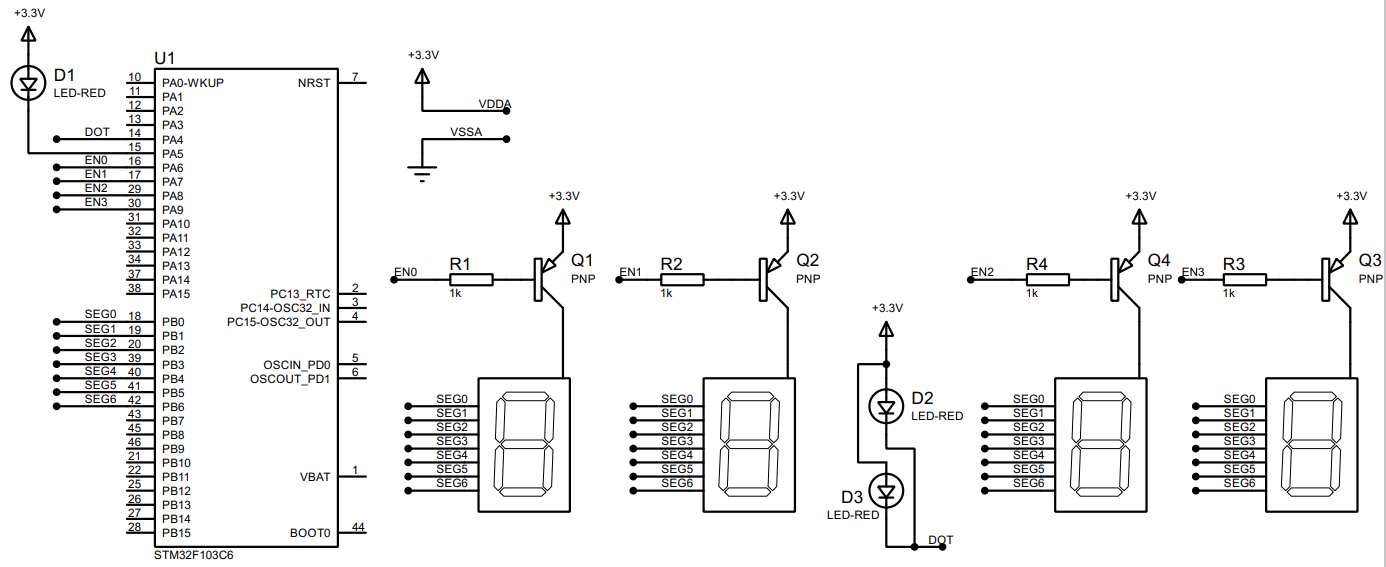
\includegraphics[width=5.5in]{graphics/lab2_ex2a.PNG}
    \caption{\textit{Simulation schematic in Proteus}}
    \label{bai2_pic1a}
\end{figure}

Blink the two LEDs every second. Meanwhile, number 3 is displayed on the third seven segment and number 0 is displayed on the last one (to present 12 hour and a half). The switching time for each seven segment LED is also a half of second (500ms). \textbf{Implement your code in the timer interrupt function.}\\

\textbf{Report 1: } Capture your schematic from Proteus and show in the report.

\begin{figure}[!htp]
    \centering
    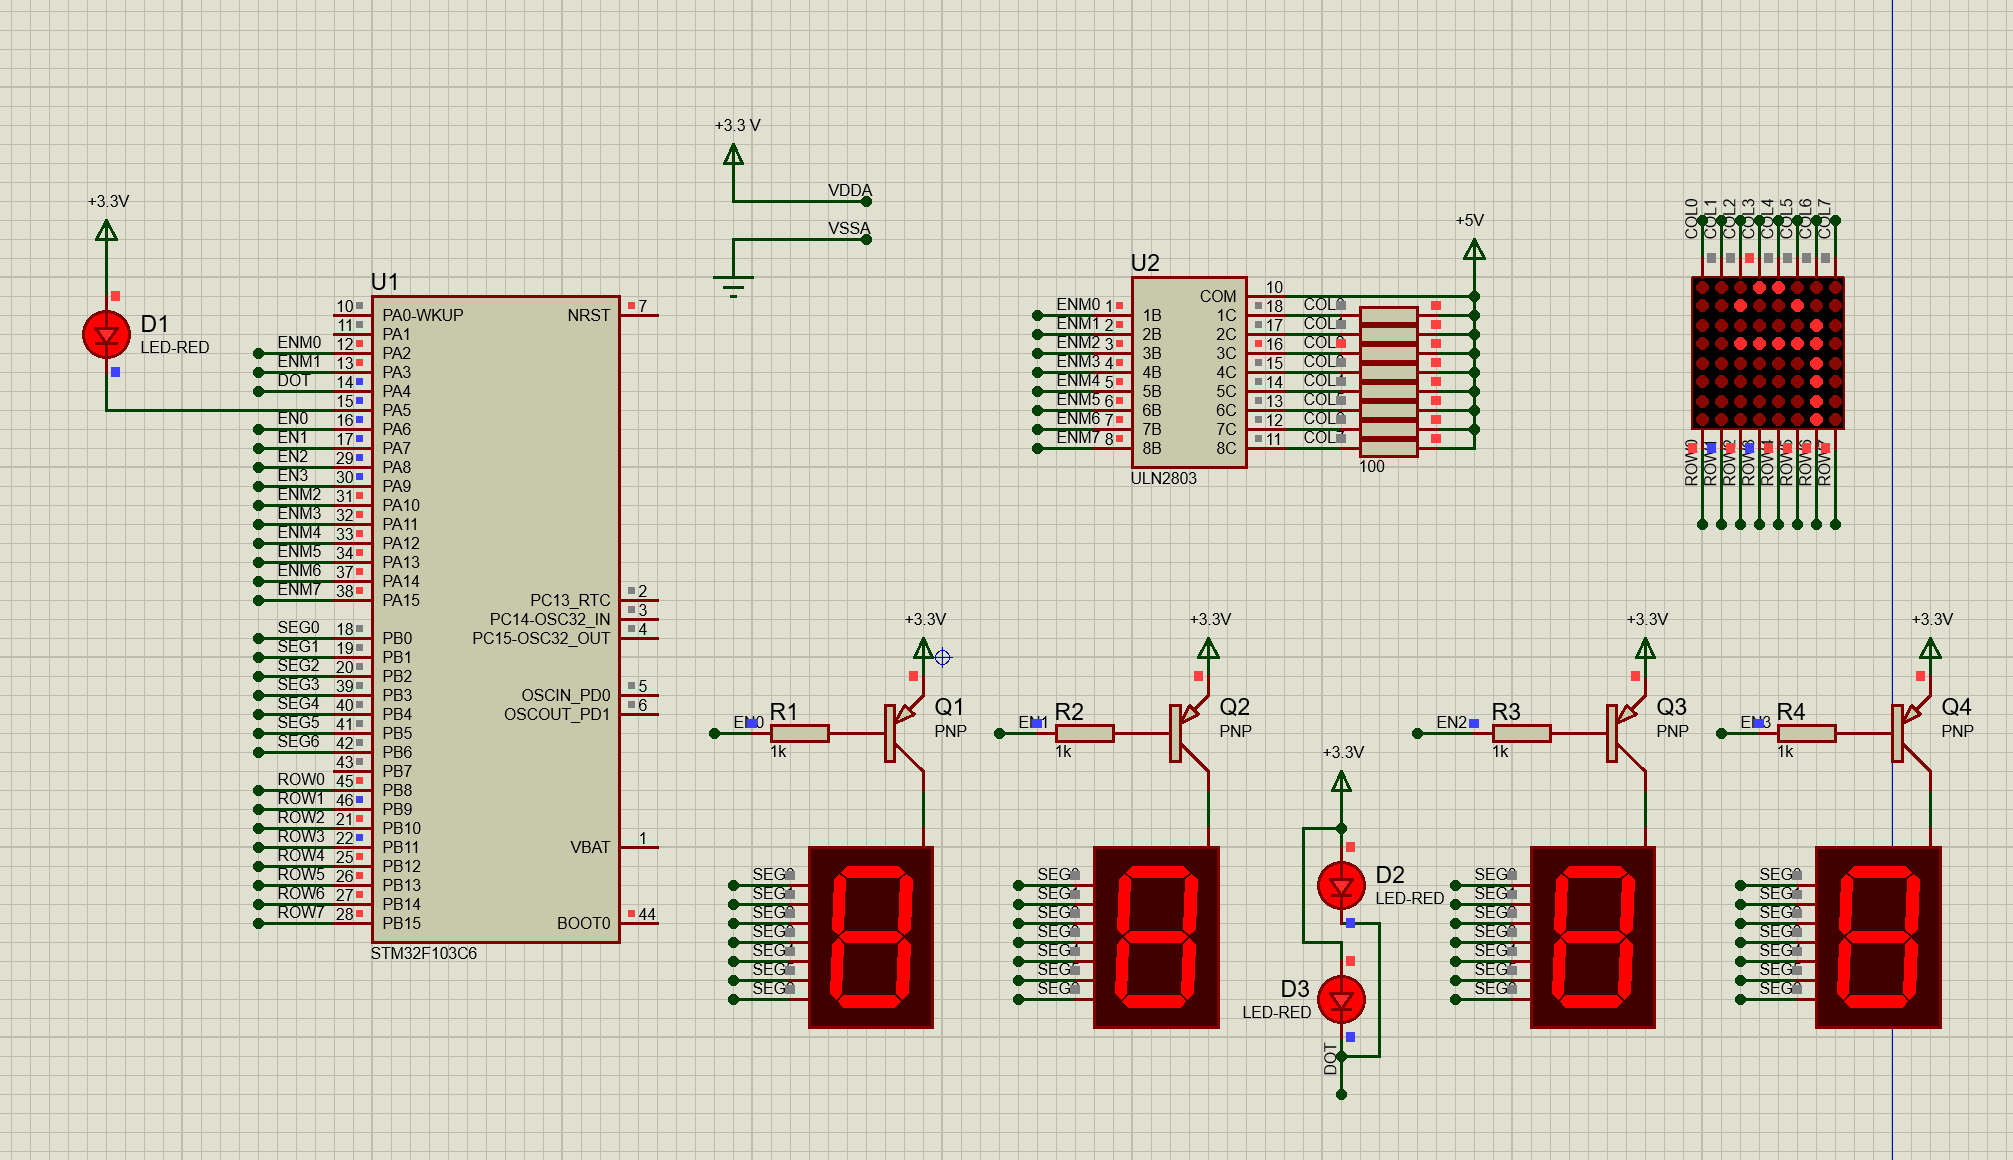
\includegraphics[width=5.5in]{graphics/f1.png}
    \caption{\textit{Schematic in Proteus}}
\end{figure}

\pagebreak

\textbf{Report 2: } Present your source code in the \textbf{HAL\_TIM\_PeriodElapsedCallback} function.\\

\begin{lstlisting}[caption=The \textbf{HAL\_TIM\_PeriodElapsedCallback} function]
#define TIME_SWITCH 50
//(x10 ms)
int counter = TIME_SWITCH;
int LED_PA5 = 100;
int state = 0;
int time_2led = 100;
void HAL_TIM_PeriodElapsedCallback(TIM_HandleTypeDef *htim)
{
	if(time_2led <= 0){
		HAL_GPIO_TogglePin(DOT_GPIO_Port, DOT_Pin);
		time_2led = 100;
	}
	if(counter <= 0){
		if(state == 0){
			HAL_GPIO_WritePin(EN3_GPIO_Port, EN3_Pin, 1);
			HAL_GPIO_WritePin(EN2_GPIO_Port, EN2_Pin, 1);
			HAL_GPIO_WritePin(EN1_GPIO_Port, EN1_Pin, 1);
			HAL_GPIO_WritePin(EN0_GPIO_Port, EN0_Pin, 0);
			display7SEG(1);
			state = 1;
		}
		else if(state == 1){
			HAL_GPIO_WritePin(EN3_GPIO_Port, EN3_Pin, 1);
			HAL_GPIO_WritePin(EN2_GPIO_Port, EN2_Pin, 1);
			HAL_GPIO_WritePin(EN1_GPIO_Port, EN1_Pin, 0);
			HAL_GPIO_WritePin(EN0_GPIO_Port, EN0_Pin, 1);
			display7SEG(2);
			state = 2;
		}
		else if(state == 2){
			HAL_GPIO_WritePin(EN3_GPIO_Port, EN3_Pin, 1);
			HAL_GPIO_WritePin(EN2_GPIO_Port, EN2_Pin, 0);
			HAL_GPIO_WritePin(EN1_GPIO_Port, EN1_Pin, 1);
			HAL_GPIO_WritePin(EN0_GPIO_Port, EN0_Pin, 1);
			display7SEG(3);
			state = 3;
		}
		else if(state == 3){
			HAL_GPIO_WritePin(EN3_GPIO_Port, EN3_Pin, 0);
			HAL_GPIO_WritePin(EN2_GPIO_Port, EN2_Pin, 1);
			HAL_GPIO_WritePin(EN1_GPIO_Port, EN1_Pin, 1);
			HAL_GPIO_WritePin(EN0_GPIO_Port, EN0_Pin, 1);
			display7SEG(0);
			state = 0;
		}
		counter = TIME_SWITCH;
	}
	if(LED_PA5 <= 0){
		 LED_PA5 = 100;
		 HAL_GPIO_TogglePin(LED_RED_GPIO_Port, LED_RED_Pin);
	 }
	counter--;
	time_2led--;
	LED_PA5--;
}
\end{lstlisting}

\textbf{Short question: } What is the frequency of the scanning process?\\
\textbf{Answer: } The frequency of the scanning process is 0.5 Hz, as each seven-segment LED is switched every half second (500 ms).
\subsection{Exercise 3}
Implement a function named \textbf{update7SEG(int index)}. An array of 4 integer numbers are declared in this case. The code skeleton in this exercise is presented as following:

\begin{lstlisting}[caption=An example for your source code]
const int MAX_LED = 4;
int index_led = 0;
int led_buffer[4] = {1, 2, 3, 4};
void update7SEG(int index){
    switch (index){
        case 0:
            //Display the first 7SEG with led_buffer[0]
            break;
        case 1:
            //Display the second 7SEG with led_buffer[1]
            break;
        case 2:
            //Display the third 7SEG with led_buffer[2]
            break;
        case 3:
            //Display the forth 7SEG with led_buffer[3]
            break;
        default:
            break;
    }
}
\end{lstlisting}

This function should be invoked in the timer interrupt, e.g update7SEG(index\_led++). The variable \textbf{index\_led} is updated to stay in a valid range, which is from 0 to 3. \\

\textbf{Report 1: } Present the source code of the update7SEG function. \\

\begin{lstlisting}[caption=The update7SEG function]
void update7SEG(int index){
			if(index >= MAX_LED || index < 0) return;
			HAL_GPIO_WritePin(EN3_GPIO_Port, EN3_Pin, index!=3);
			HAL_GPIO_WritePin(EN2_GPIO_Port, EN2_Pin, index!=2);
			HAL_GPIO_WritePin(EN1_GPIO_Port, EN1_Pin, index!=1);
			HAL_GPIO_WritePin(EN0_GPIO_Port, EN0_Pin, index!=0);
			display7SEG(led_buffer[index]);
}
\end{lstlisting}

\textbf{Report 2: } Present the source code in the HAL\_TIM\_PeriodElapsedCallback.\\

\begin{lstlisting}[caption=The update7SEG function]
#define TIME_SWITCH 50
//(x10 ms)
int counter = TIME_SWITCH;
int LED_PA5 = 100;
int time_2led = 100;

void HAL_TIM_PeriodElapsedCallback(TIM_HandleTypeDef *htim)
{
	if(time_2led <= 0){
		HAL_GPIO_TogglePin(DOT_GPIO_Port, DOT_Pin);
		time_2led = 100;
	}
	if(counter <= 0){
		update7SEG(index_led++);
		if(index_led > 3) index_led = 0;
		counter = TIME_SWITCH;
	}
	if(LED_PA5 <= 0){
		 LED_PA5 = 100;
		 HAL_GPIO_TogglePin(LED_RED_GPIO_Port, LED_RED_Pin);
	 }
	LED_PA5--;
	counter--;
	time_2led--;
}
\end{lstlisting}

Students are proposed to change the values in the \textbf{led\_buffer} array for unit test this function, which is used afterward.

\subsection{Exercise 4}
Change the period of invoking update7SEG function in order to set the frequency of 4 seven segment LEDs to 1Hz. The DOT is still blinking every second.\\


\textbf{Report 1: } Present the source code in the \textbf{HAL\_TIM\_PeriodElapsedCallback}. \\

\begin{lstlisting}[caption=source code in the \textbf{HAL\_TIM\_PeriodElapsedCallback}]
#define TIME_SWITCH 25
//(x10 ms)
int counter = TIME_SWITCH;
int LED_PA5 = 100;
int time_2led = 100;

void HAL_TIM_PeriodElapsedCallback(TIM_HandleTypeDef *htim)
{
	if(time_2led <= 0){
		HAL_GPIO_TogglePin(DOT_GPIO_Port, DOT_Pin);
		time_2led = 100;
	}
	if(counter <= 0){
		update7SEG(index_led++);
		if(index_led > 3) index_led = 0;
		counter = TIME_SWITCH;
	}
	if(LED_PA5 <= 0){
		 LED_PA5 = 100;
		 HAL_GPIO_TogglePin(LED_RED_GPIO_Port, LED_RED_Pin);
	 }
	LED_PA5--;
	counter--;
	time_2led--;
}
\end{lstlisting}

\subsection{Exercise 5}
Implement a digital clock with \textbf{hour} and \textbf {minute} information displayed by 2 seven segment LEDs. The code skeleton in the \textbf{main} function is presented as follows:
\begin{lstlisting}[caption=An example for your source code]
int hour = 15, minute = 8, second = 50;

while(1){
    second++;
    if (second >= 60){
        second = 0;
        minute++;
    }
    if(minute >= 60){
        minute = 0;
        hour++;
    }
    if(hour >=24){
        hour = 0;
    }
    updateClockBuffer();
    HAL_Delay(1000);
}
\end{lstlisting}

The function \textbf{updateClockBuffer} will generate values for the array \textbf{led\_buffer} according to the values of hour and minute. In the case these values are 1 digit number, digit 0 is added. \\

\textbf{Report 1: } Present the source code in the \textbf{updateClockBuffer} function.

\begin{lstlisting}[caption=The update7SEG function]
#define TIME_SWITCH 25
//(x10 ms)
int counter = TIME_SWITCH;
int time_2led = 25;
int hour = 15, minute = 59, second = 50;

void updateClockBuffer(){
if(hour > 99 || hour < 0 || minute > 99 || minute < 0) return;
led_buffer[0] = hour/10;
led_buffer[1] = hour%10;
led_buffer[2] = minute/10;
led_buffer[3] = minute%10;
}
\end{lstlisting}

\subsection{Exercise 6}
The main target from this exercise to reduce the complexity (or reduce code processing) in the timer interrupt. The time consumed in the interrupt can lead to the nested interrupt issue, which can crash the whole system. A simple solution can disable the timer whenever the interrupt occurs, the enable it again. However, the real-time processing is not guaranteed anymore.\\

In this exercise, a software timer is created and its counter is count down every timer interrupt is raised (every 10ms). By using this timer, the \textbf{Hal\_Delay(1000)} in the main function is removed. In a MCU system, non-blocking delay is better than blocking delay. The details to create a software timer are presented bellow. The source code is added to your current program, \textbf{do not delete the source code you have on Exercise 5.}\\

\textbf{Step 1: } Declare variables and functions for a software timer, as following:
\begin{lstlisting}[caption=Software timer based timer interrupt]
/* USER CODE BEGIN 0 */
int timer0_counter = 0;
int timer0_flag = 0;
int TIMER_CYCLE = 10;
void setTimer0(int duration){
	timer0_counter = duration /TIMER_CYCLE;
	timer0_flag = 0;
}
void timer_run(){
	if(timer0_counter > 0){
		timer0_counter--;
		if(timer0_counter == 0) timer0_flag = 1;
	}
}
/* USER CODE END 0 */
\end{lstlisting}

Please change the \textbf{TIMER\_CYCLE} to your timer interrupt period. In the manual code above, it is \textbf{10ms}. \\

\textbf{Step 2: } The \textbf{timer\_run()} is invoked in the timer interrupt as following:

\begin{lstlisting}[caption=Software timer based timer interrupt]
void HAL_TIM_PeriodElapsedCallback(TIM_HandleTypeDef *htim){
	
	timer_run();
	
	//YOUR OTHER CODE
}
\end{lstlisting}

\textbf{Step 3: } Use the timer in the main function by invoked setTimer0 function, then check for its flag (timer0\_flag). An example to blink an LED connected to PA5 using software timer is shown as follows:
\begin{lstlisting}[caption=Software timer is used in main fuction to blink the LED]
setTimer0(1000);
while (1){
    if(timer0_flag == 1){
        HAL_GPIO_TogglePin(LED_RED_GPIO_Port, LED_RED_Pin);
        setTimer0(2000);
    }
}
\end{lstlisting}

\textbf{Report 1: } if in line 1 of the code above is miss, what happens after that and why?\\

\textbf{Answer: } If line 1 is missed, the LED will not blink as expected. The reason is the flag not set to 1 before checking it in the while loop because miss line 1 to call function setTimer0 to set the timer0\_counter to a non-zero value. As a result, the condition in the if statement (timer0\_flag == 1) will never be true, and the LED will not toggle its state.

\textbf{Report 2: } if in line 1 of the code above is changed to setTimer0(1), what happens after that and why?\\

\textbf{Answer: } The LED will not blink as expected because the flag still not set to 0 after line 1 in function runs. The reason is paramater in line 1 is 0, so the function timer\_run() will not decrease the timer0\_counter, and the flag will not be set to 1. As a result, the condition in the if statement (timer0\_flag == 1) will never be true, and the LED will not toggle its state.

\textbf{Report 3: } if in line 1 of the code above is changed to setTimer0(10), what is changed compared to 2 first questions and why?\\

\textbf{Answer: } The LED will blink as expected but it initially run faster than expected.

\subsection{Exercise 7}
Upgrade the source code in Exercise 5 (update values for hour, minute and second) by using the software timer and remove the HAL\_Delay function at the end. Moreover, the DOT (connected to PA4) of the digital clock is also moved to main function. \\

\textbf{Report 1: } Present your source code in the while loop on main function.

\begin{lstlisting}[caption= the while loop on main function]
  setTimer(0, 1000); //RED_LED
  setTimer(1, 7); //CLOCK HOUR_MINUTE_SECOND
  setTimer(2, 250); //DISLAY 7 - SEG LED
  setTimer(3, 500);
	while (1){
	if(istimer_flag(0) == 1){
		   HAL_GPIO_TogglePin(LED_RED_GPIO_Port, LED_RED_Pin);
		   setTimer(0, 2000);
	  }
	  if(istimer_flag(1) == 1){
		  second++;
		  if (second >= 60){
			  second = 0;
			  minute++;
		  }
		  if(minute >= 60){
			  minute = 0;
			  hour++;
		  }
		  if(hour >=24){
			  hour = 0;
		  }
		  updateClockBuffer();
		  setTimer(1, 1000);
	  }
	  if(istimer_flag(2) == 1){
		  update7SEG(index_led++);
		  if(index_led > 3) index_led = 0;
		  setTimer(2, 250);
	  }
	  if(istimer_flag(3) == 1){
		  HAL_GPIO_TogglePin(DOT_GPIO_Port, DOT_Pin);
		  setTimer(3, 1000);
	  }
  }
\end{lstlisting}

\subsection{Exercise 8}
Move also the update7SEG() function from the interrupt  timer to the main. Finally, the timer interrupt only used to handle  software timers. All processing (or complex computations) is move to an infinite loop on the main function, optimizing the complexity of the interrupt  handler function.\\

\textbf{Report 1: } Present your source code in the the main function. In the case more extra functions are used (e.g. the second software timer), present them in the report as well.

\begin{lstlisting}[caption= the while loop on main function]
  setTimer(0, 1000); //RED_LED
  setTimer(1, 7); //CLOCK HOUR_MINUTE_SECOND
  setTimer(2, 250); //DISLAY 7 - SEG LED
  setTimer(3, 500);
	while (1)
  {
	if(istimer_flag(0) == 1){
		   HAL_GPIO_TogglePin(LED_RED_GPIO_Port, LED_RED_Pin);
		   setTimer(0, 2000);
	  }
	  if(istimer_flag(1) == 1){
		  second++;
		  if (second >= 60){
			  second = 0;
			  minute++;
		  }
		  if(minute >= 60){
			  minute = 0;
			  hour++;
		  }
		  if(hour >=24){
			  hour = 0;
		  }
		  updateClockBuffer();
		  setTimer(1, 1000);
	  }
	  if(istimer_flag(2) == 1){
		  update7SEG(index_led++);
		  if(index_led > 3) index_led = 0;
		  setTimer(2, 250);
	  }
	  if(istimer_flag(3) == 1){
		  HAL_GPIO_TogglePin(DOT_GPIO_Port, DOT_Pin);
		  setTimer(3, 1000);
	  }
  }
\end{lstlisting}

\subsection{Exercise 9}

This is an extra works for this lab. A LED Matrix is added to the system. A reference design is shown in figure bellow:
\begin{figure}[!htp]
    \centering
    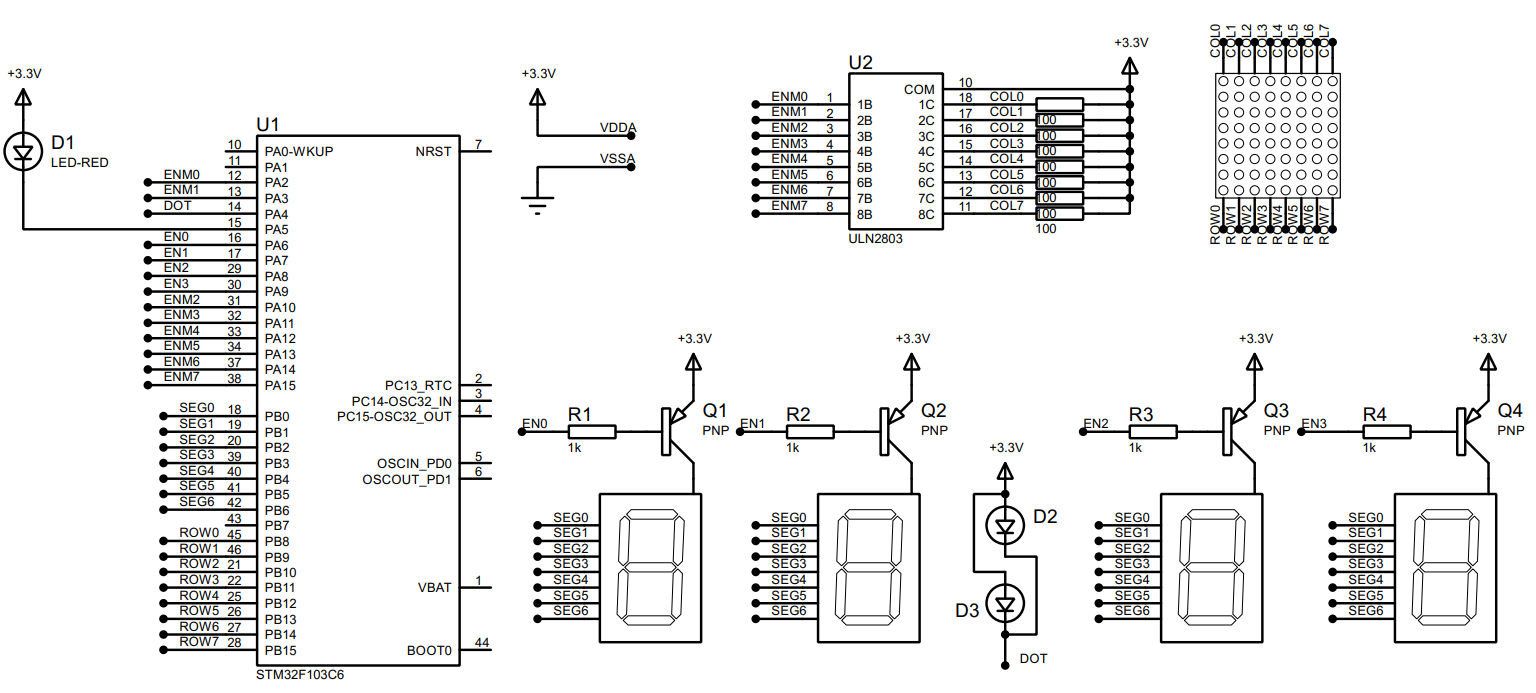
\includegraphics[width=5.5in]{graphics/lab2_m4.PNG}
    \caption{\textit{LED matrix is added to the simulation}}
    \label{bai2_pic9}
\end{figure}

In this schematic, two new components are added, including the \textbf{MATRIX-8X8-RED} and \textbf{ULN2803}, which is an NPN transistor array to enable the power supply for a column of the LED matrix. Students can change the enable signal (from ENM0 to  ENM7) if needed. Finally, the data signal (from ROW0 to ROW7) is connected to PB8 to PB15. \\

\textbf{Report 1: } Present the schematic of your system by capturing the screen in Proteus.\\

\begin{figure}[!htp]
	\centering
	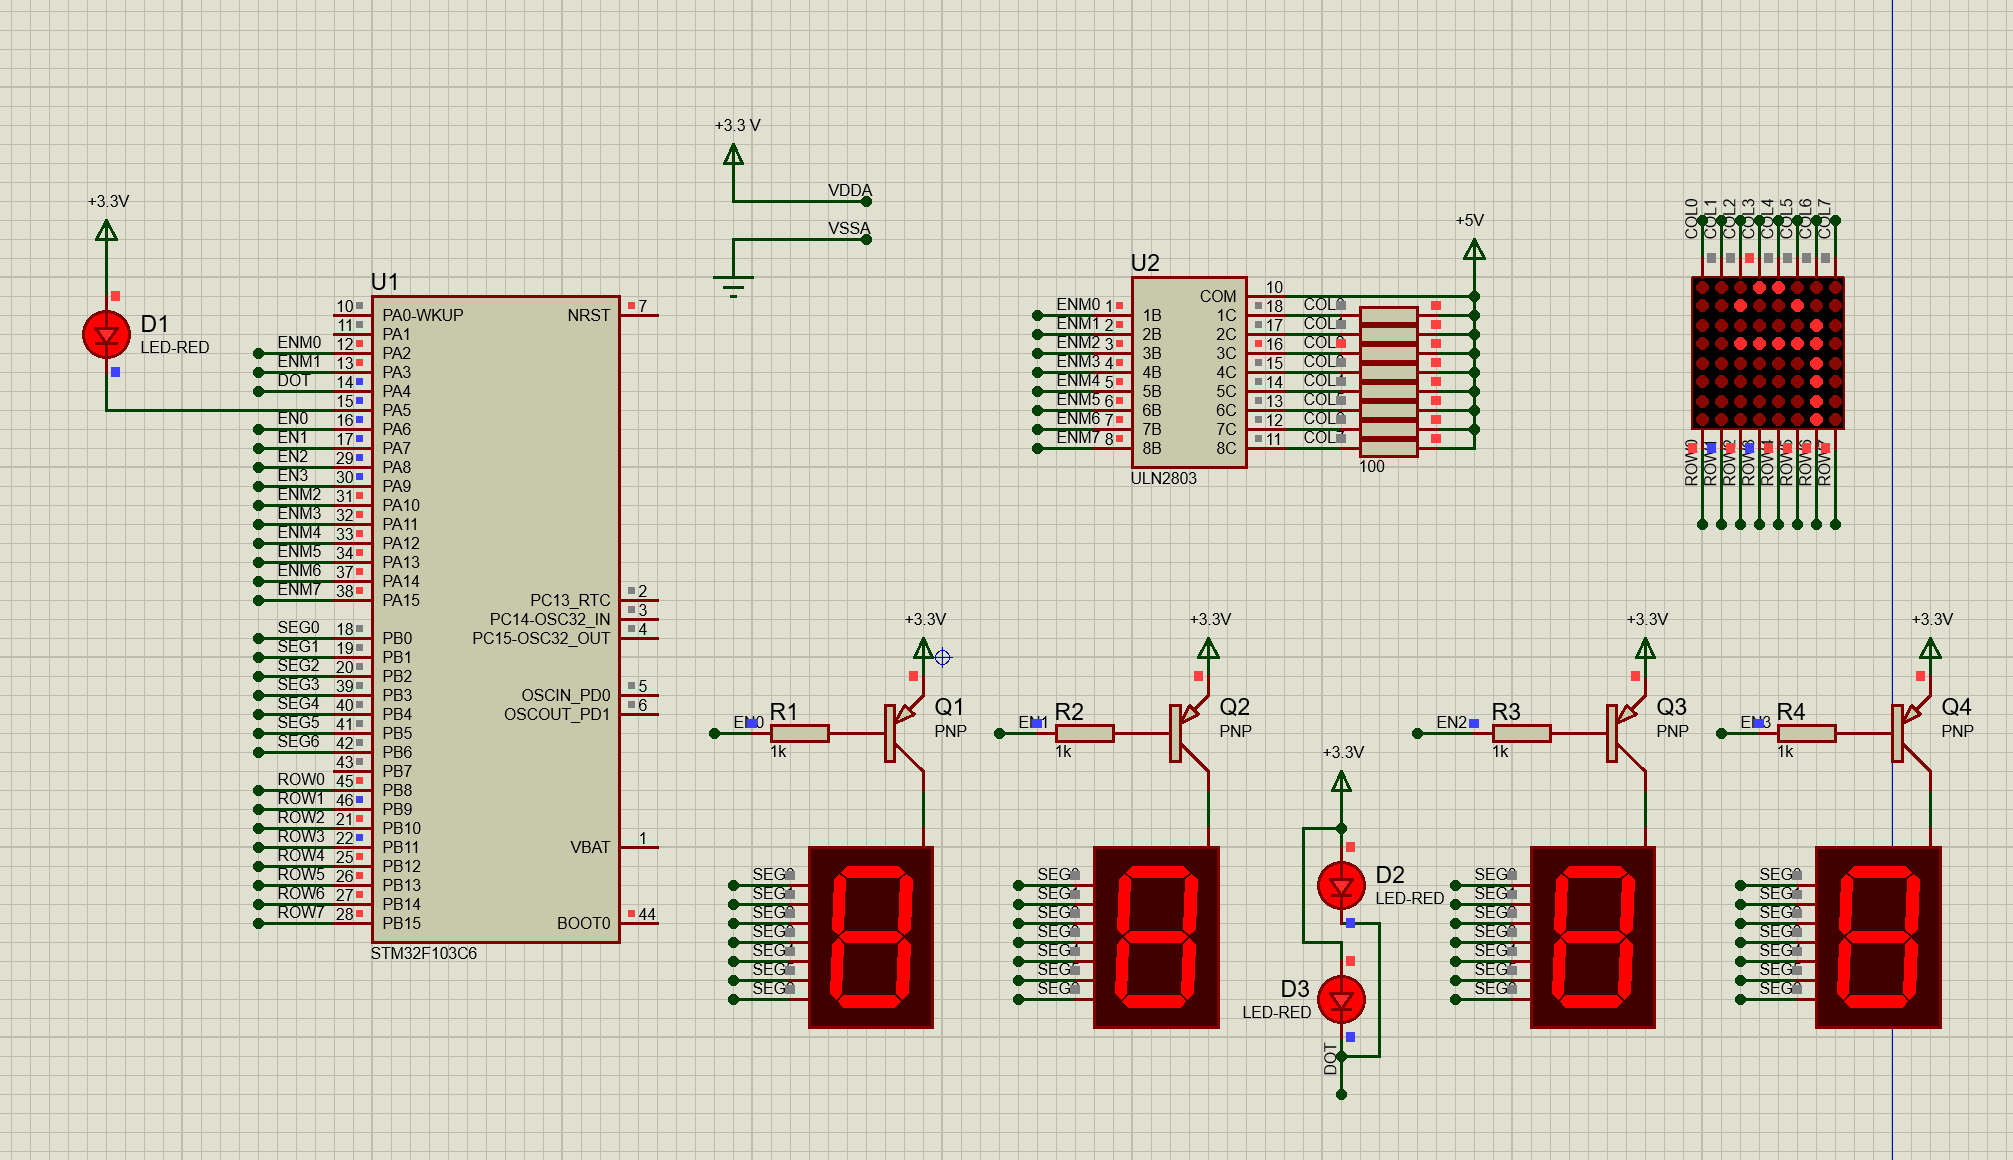
\includegraphics[width=5.5in]{graphics/f1.png}
	\caption{\textit{Schematic in Proteus}}
\end{figure}
\textbf{Report 2: } Implement the function, updateLEDMatrix(int index), which is similarly  to 4 seven led segments.

\begin{lstlisting}[caption=Function to display data on LED Matrix]
 const int MAX_LED_MATRIX = 8;
 uint8_t matrix_buffer[8] = { 0x00, 0xFC, 0x0A, 0x09, 0x09, 0x0A, 0xFC, 0x00};
 int index_led_matrix = 0;
//USING THIS CODE IF ONLY THIS LAB BECAUSE THEIR ARE SAME PORT
uint16_t Pin_LED_Maxtrix[8] = {ENM0_Pin,ENM1_Pin,ENM2_Pin,ENM3_Pin,ENM4_Pin,ENM5_Pin,ENM6_Pin,ENM7_Pin};
 void updateLEDMatrix(int index){
	if(index >= MAX_LED_MATRIX || index < 0) return;
	HAL_GPIO_WritePin(ENM0_GPIO_Port, ENM0_Pin | ENM1_Pin | ENM2_Pin | ENM3_Pin | ENM4_Pin | ENM5_Pin | ENM6_Pin | ENM7_Pin, SET);
	uint16_t matrix_pin_for_buffer0 = matrix_buffer[index];
	uint16_t matrix_pin_for_buffer1 = ~matrix_buffer[index];
	matrix_pin_for_buffer0 = matrix_pin_for_buffer0<<8;
	matrix_pin_for_buffer1 = matrix_pin_for_buffer1<<8;
	HAL_GPIO_WritePin(ROW0_GPIO_Port, matrix_pin_for_buffer0, 0);
	HAL_GPIO_WritePin(ROW0_GPIO_Port, matrix_pin_for_buffer1, 1);
	HAL_GPIO_WritePin(ENM0_GPIO_Port, Pin_LED_Maxtrix[index], RESET);

  }
\end{lstlisting}

Student are free to choose the invoking frequency of this function. However, this function is supposed to invoked in main function. Finally, please update the \textbf{matrix\_buffer} to display character \textbf{"A"}.

\subsection{Exercise 10}
Create an animation on LED matrix, for example, the character is shifted to the left. 

\textbf{Report 1: } Briefly describe your solution and present your source code in the report.

Change the buffer to create the animation effect shift character "A" down. The code is presented as follows:
\begin{lstlisting}[caption= the while loop on main function]
	  setTimer(0, 100);
while (1){
	if(istimer_flag(0) == 1){
		  matrix_buffer[index_led_matrix] = matrix_buffer[index_led_matrix]<<1|matrix_buffer[index_led_matrix]>>7;
		  updateLEDMatrix(index_led_matrix--);
		  if(index_led_matrix < 0) {index_led_matrix = 7;}
		  setTimer(0, 10);
	  }
  }
\end{lstlisting}

\pagebreak
\section*{References}
% \addcontentsline{toc}{section}{References}
% \bibliographystyle{plainnat} % Reference style
% \bibliography{references} % .bib file containing references
\end{document}